% \documentclass[11pt]{scrartcl}
\documentclass[english,mgr,shortabstract]{iithesis}

% \RedeclareSectionCommand[
%   indent=1em]{subsubsection}
% \addtokomafont{subsubsection}{\textbf}

% \usepackage{amsmath,amssymb,amsfonts,amsthm,mathtools}
\usepackage{color}
\usepackage{listings}
\usepackage{fontspec}
% \usepackage{mathptmx}
% \usepackage[scaled=.90]{helvet}

\definecolor{keywords}{RGB}{30,200,30}
\definecolor{comments}{RGB}{210,40,40}
\lstset{
  basicstyle=\ttfamily,
  showstringspaces=false
}

% \usepackage{bbm}
\usepackage{graphicx}
\usepackage{url}
\usepackage{dirtytalk}
\usepackage{csquotes}
\SetBlockThreshold{0}

\usepackage{wrapfig}

\usepackage{caption}

\usepackage{xcolor}
\let\cleardoublepage\clearpage

\newcommand*{\figref}[1]{[\textbf{\figurename}~\ref{#1}]}

\englishtitle{The application of functional programming to~the~construction of~a~visual
  programming environment}
\englishabstract{
  Traditional programming methods are becoming increasingly disconnected from
  modern input methods, like touchscreens. An alternative --- programming with
  diagrams, called Visual Programming Languages, has long existed, but received little
  attention. This
  thesis uses ideas inspired by functional programming to propose an approach to
  representation of the Clojure programming language,
  that allows manipulation of program both as a text and as a diagram. This
  approach is implemented as a Visual Programming Editor --- Jarvis.
}
\polishtitle{Zastosowanie funkcyjnego paradygmatu do tworzenia graficznego środowiska programistycznego}
\polishabstract{
  Tradycyjne metody programowania wymuszają komunikację z komputerem poprzez
  klawiaturę i myszkę --- sprzęt obecnie coraz częściej zastepowany przez ekrany dotykowe.
  Od wielu lat istnieje alternatywa --- wizualne języki programowania. Ten sposób jednak
  z wielu przyczyn nie
  zdobył dużej popularności. Ta praca pokazuje sposób eliminacji jego
  mankamentów poprzez wykorzystanie programowania funkcyjnego, oraz implementuje
  nowe wizualne środowisko programistyczne --- Jarvis.
}
\advisor{dr hab. Dariusz Biernacki}
\author{Łukasz Czapliński}
\date{\today}

\begin{document}
\maketitle

\chapter{Introduction}
\section{Visual Programming Languages (VPLs)}
Programming is an art of communication --- both with a machine and with other
people.
To express algorithms in a machine-readable way, we use programming languages.
When it comes to describing our ideas to other programmers, we often use
entirely different means.
Diagrams are one of the most universal ones.
Since the invention of graphical interfaces, we have been trying to apply
similar means to communicating with the machine.

Visual Programming Languages are one of many attempts to achieve this.
Shapes, colours and text annotations are used to represent computer programs,
instead of employing only formatted text.
That representation is ``first-class'' --- users are expected to manipulate it
directly, instead of changing some underlying text representation.
Such programming languages often do not possess human-readable textual
representation.
There is no widely adopted formal definition of a VPL.
The one most fitting in context of this thesis is:
\blockquote{Interactive use of diagrams
  in the process of programming~\cite[Chapter 2]{nickerson1995visual}.}


Attempts to create such language were possible only after the invention of
graphical interface.
The first interactive visual programming language was created by W. Sutherland
in 1966~\cite{firstVPL}.
A simple language based on flowcharts was created in 1969 at Rand~\cite{grail}.
After the invention of the first visual programming environments at Xerox Parc in
1970, the main focus of the next generations was to improve the interface for
programmers, while still using textual representation.
It is visible in most programming environments, from Smalltalk to Microsoft
Visual Studio.
No visual programming language has ever gained traction comparable to common textual
programming languages.


Historical reasons for that are twofold.
First of all, although it might be easier for a novice to understand the idea of
an algorithm from a diagram, there are no gains for an experienced programmer.
For a completely new paradigm to gain traction, current programmers would have
to learn it.
This would be even more painful than learning a new programming language, as
syntax of most mainstream languages with textual representation is similar.

Additionally, most of programming tools are specialised for text manipulation.
If a language is text-based, it can easily be presented, edited, stored and
transmitted by a multitude of different programs. If, on the other hand, a program
is a diagram which can only be rendered by a specialised editor, it becomes
much harder to collaborate on it with a group of people, and much harder to
share it with other programmers.

\section{Visual Programming Environments (VPEs)}
Since the invention of Smalltalk, programming environments that married textual
representation with graphical interface have been becoming more and more
popular.
Nowadays, powerful integrated development environments (IDEs), such as Visual
Studio (\url{https://www.visualstudio.com/}) or IntelliJ IDEA
(\url{https://www.jetbrains.com/idea/}) are commonly used.

Their main advantage over visual programming languages is their versatility ---
textual representation has allowed them to gain popularity without forcing existing
programmers to change habits, and to keep tools that support text.
Their chief disadvantage is the lack of flexibility. They are blurring the lines between
the editor and the language ---
because new language features need new editor features, and so new IDEs dwarf
the venerable
Emacs (which was often accused of being nothing short of operating system).
At the same time, textual representation forces keyboard and doesn't
allow experimenting with new input methods. Even the interaction with mouse is only a secondary mean
of interacting with the editor. This stands in stark contrast with how user
interfaces are evolving right now.

Nowadays, touchscreens are getting more and more attention --- they are currently
the prime interface for smartphones.
Thus, most young people are more familiar with them, and not mouse or keyboard.
Text is easy to manipulate with keyboard, but hard to manipulate with gestures ---
visual programming would be far more intuitive for new adepts.

In addition, programming is becoming less of an arcane discipline, and more of
a skill needed in every branch of industry.
This makes collaboration between programmers and domain experts even more
important.
The ease of understanding diagrams (and not a specialised programming language) might become a
crucial factor in application development, decreasing production time.

\section{About this work}
The purpose of this thesis is to address the fundamental problem with Visual
Programming Languages: collaboration between the programmer using visual
programming editor, and the one with a standard text editor. This might lead to
more widespread use of ``programming with diagrams,'' and better adoption of
touch-based input methods in programming, which can potentially revolutionize
how programmers work.
The main idea is to keep a program encoded as text, but visualize and modify
it as a diagram. In order to achieve this, the amount of syntactic structures in
the text is reduced by adopting a language from the field of functional programming.

First, functional programming is introduced, along with the LISP approach to
language design. Then, a dialect of LISP --- Clojure --- is presented, along
with the editor features that make working with this language easy.
In  following chapters we present its
visual representation in Jarvis --- the editor which is the main achievement
of this thesis. Jarvis is then described in detail --- both what writing
programs in it looks like, and how it is implemented.
It is then compared with both other VPLs and traditional
Clojure editors in order to better explain in what it excels.


\chapter{Functional Programming}
\section{What is functional programming?}
Functional programming can be defined as:
\blockquote{Paradigm of programming where
  fundamental operation is the application of functions to
  arguments~\cite{Hughes:1989:WFP:63410.63411}.}

It means that the program itself is a function which treats its environment as
an input and delivers some changes to outside world as a result.
The main function is composed of auxiliary functions, which are in turn defined
as a composition of other functions.
This ``functions all the way down'' approach (down to a handful of language
primitives) leads to very powerful and concise languages.
This is caused by better code modularisation in form of higher order functions.
It bears resemblance to structured programming being superior to imperative
programming.
The presence of GOTOs made it impossible to generalise programs (as labels were
local and impossible to encapsulate).
Functional programming forbids variable mutation (or more generally, side
effects).
The only possible declarations are static assignments.
Mutable states are encapsulated in specialised structures.
This facilitates code analysis.
Unfortunately, it doesn't come without downsides: it’s hard for an average
programmer to switch to functional programming.


\section{How can this be applied to VPL design?}

Ideally, a suitable textual representation for VPL would be flexible, powerful
and simple.
One kind of functional programming languages fits this description especially
well.
It is LISP (LISt Processor), developed by the Artificial Intelligence group at
M.I.T~\cite{recursive}.

It is based on Symbolic Expressions (S-expressions) and functions operating on
them.
Briefly, an S-expression is a list of primitives and S-expressions.
A list containing primitives \lstinline|a, b, c| is represented as \lstinline|(a, b, c)|.
S-functions are functions operating on S-expressions, encoded as S-expressions.
LISP is just an interpreter for S-functions.
It’s remarkable, because encoding language in the same way as its data
structures empowers it.
For example, one can easily write a function that operates on syntactic forms
instead of values.
This makes the language very powerful, while keeping the syntax absolutely minimal.
The price for generalised syntax is plenty of similar structures in the program and
results in a code that is hard to read:

\begin{lstlisting}
(defun fibonacci (N)
  "Compute the Nth Fibonacci number."
  (if (or (zerop N) (= N 1))
    1
    (+ (fibonacci (- N 1)) (fibonacci (- N 2)))))
\end{lstlisting}

\chapter{Clojure}
\section{Introduction}
Clojure is a modern functional programming language based on LISP.\@It’s
described as:

\blockquote{Clojure is a dynamic, general-purpose
  programming language, combining the approachability and interactive
  development of a scripting language with an efficient and robust
  infrastructure for multithreaded programming. Clojure is a dialect of Lisp,
  and shares with Lisp the code-as-data philosophy and a powerful macro
  system~\cite{clojure_website}.}

\section{Syntax}
Lisp’s code-as-data philosophy means that Clojure programs are built using its
data structures.
Generally, Clojure’s specification~\cite{clojure_spec} defines Extensible Data Notation
(EDN), which is a description of data structures available to Clojure
programmers.
It includes the following primitives:
\begin{itemize}
  \item Nil
  \item Booleans
  \item Integers
  \item Floats
  \item Characters
  \item Strings
  \item Symbols
  \item Keywords
\end{itemize}
In addition to them, it defines a few compound types, encoded as S-expressions:
\begin{itemize}
  \item List --- \lstinline$(a b c) $
  \item Vector --- \lstinline$[a b c]$
  \item Map --- \lstinline|{a_key a_value b_key b_value}|
  \item Set --- \lstinline$#{a b c}$
\end{itemize}
Extensibility is achieved by tags~\cite{edn_format}. Any element can be
prefixed by a tag, for example:
\begin{lstlisting}
#myapp/Person {:first "Fred" :last "Mertz"} 
\end{lstlisting}
When Clojure’s parser encounters such an element, it has a couple of choices, one
of them being creating a known representation.
This, coupled with the fact that only elements readable by Clojure’s parser can
be tagged, means that the parser that doesn’t know a specific tag can still work
on a Clojure program containing that tag.


\section{Semantics}

\subsubsection{Evaluation}
Everything but non-empty lists and symbols evaluate to corresponding data
structure.
Symbols are resolved, which generally means a lookup for a variable corresponding
to that symbol.
Non-empty lists are interpreted as calls in form of \lstinline|(operator operands*)|.
Whether operands are evaluated, depends on the type of the operator.
These include:
\begin{itemize}
  \item Special forms, which are Clojure’s primitives. There are  less than 20
    in total.
  \item Macros, which are used to manipulate syntactic abstractions. Operands
    are passed unevaluated to the macro, and the returned data structure is then
    evaluated.
\end{itemize}
If operator is neither a special form nor a macro, the form is interpreted as a
function call: both the operator and the operands are evaluated, and the
function resulting from the operator’s evaluation is called with the results of
evaluating the operands as arguments.
The returned value is the value of the expression.

\subsubsection{Data Structures}
Clojure designers opted for integrating more data structures into the syntax to
allow encoding complex data structures in a human-readable way.
One could easily build a hashmap using a constructor function
\lstinline$(hashmap a b c d)$, although using Clojure’s syntax ---
\lstinline${a b c d}$ --- is more readable and doesn’t require eval.
Also, it might be worth noting that almost all Clojure data structures are
immutable.

\subsubsection{Macro Operators}
Clojure differs from pure LISP in one more aspect.
Its reader recognises some operators and automatically transforms them:
\begin{itemize}
  \item \lstinline|@| --- dereference:
\lstinline|@some_ref| $\Rightarrow$ \lstinline|(deref some_ref)|
Used to extract value from references and atoms
  \item \lstinline|'| --- quote:
\lstinline|'foo| $\Rightarrow$ \lstinline|(quote foo)|
Works like a LISP quote, makes it possible to stop evaluation of the data structure.
  \item \lstinline|`| --- syntactic quote:
no macro equivalent.
Extends quote capabilities to allow escaping (i.e.\ evaluating only some parts of
quoted data structure).

  \item \lstinline|~| --- syntactic quote escape:
no macro equivalent.
Used in conjunction with syntactic quote:
\begin{itemize}
  \item \lstinline|`~x| $\Rightarrow$ \lstinline|x|
  \item \lstinline|`(x ~y)|
  $\Rightarrow$ \texttt{(list (quote x) y)}
\end{itemize}
\end{itemize}

\chapter{Clojure programming}
\section{Contemporary editors}
Despite Lisp syntax being hard for newcomers to understand, Clojure is
considered one of the most efficient languages for programmers.
Two factors are responsible for that: functional programming and integration
with REPL.\@
Virtues of the former were described in the previous chapters, the latter will
be discussed in this one.
REPL stands for Read-Eval-Print Loop.
Much like command line shell, or interactive shells in other languages, it
allows the programmer to send the code he’s been working on and observe the
results directly, without having to execute the whole program.
The main difference is what can be read and what can be executed.
Due to Lisp’s syntax, Clojure’s REPL can read, eval and print arbitrary
S-expression.
Non-Lisp interactive shells need to differentiate between expressions and
statements, which can lead to non-intuitive behavior.
The second difference is integration with editors.
It’s common for Clojure programmers to have an editor integration, which allows
them to send arbitrary parts of the currently edited file to REPL and observe
the results.
This results in better understanding of the language and less bugs (due to ideally
every part of code being tested during writing).


\section{Editing}
\label{sec:editing}
As mentioned previously, Clojure is edited as text.
Due to the nature of S-expressions, this can prove difficult (keeping so many
brackets paired can be troublesome).
To mitigate this, most Clojure editors provide special shortcuts which help in
editing S-expressions.

\subsubsection{Slurp}
Slurp adds an element to current S-expression by extending the parentheses one element
to the right (forwards) or left (backwards).

\begin{itemize}
\item forward: \lstinline|(1 2 [])  3| $\Rightarrow$ \lstinline|(1 2 3 [])|
\item backward: \lstinline|1 ([] 2 3)| $\Rightarrow$ \lstinline|([] 1 2 3)|
\end{itemize}
(\lstinline{[]} is the current position of the cursor.)

\subsubsection{Barf}
Barf is opposite to slurp --- it removes an element from current S-expression by
moving the parentheses left (forwards) or right (backwards).
\begin{itemize}
\item forward: \lstinline|(1 2 3 [])| $\Rightarrow$ \lstinline|(1 2 [])  3|
\item backward: \lstinline|([] 1 2 3)| $\Rightarrow$ \lstinline|1 ([] 2 3)|
\end{itemize}

\subsubsection{Transpose}
Transpose re-orders element in the current S-expression by swapping the element before
cursor with the one after.
\begin{itemize}
\item \lstinline|(1 [] 2)| $\Rightarrow$ \lstinline|(2 [] 1)|
\end{itemize}

\subsubsection{Wrap}
Wrap simply wraps the current element in the parentheses.

\begin{itemize}
\item \lstinline|println[]| $\Rightarrow$ \lstinline|(println[])|
\end{itemize}

\subsubsection{Unwrap}
Unwrap removes the parentheses from the current S-expression.
\begin{itemize}
  \item \lstinline|(println[])| $\Rightarrow$ \lstinline|println[]|
\end{itemize}

It is mostly used to inline expressions:
\begin{itemize}
  \item \lstinline|(println (1 2 3 []))| $\Rightarrow$
    \lstinline|(println 1 2 3[])|
\end{itemize}

The pain of editing S-expressions can be largely mitigated by not manipulating
text.
When S-expressions are structured visually, editing them might be as easy as
drawing a new arrow or moving a box.
This would largely remove problems with the syntax and allow programmers to focus on
the semantics of the program.


\chapter{Jarvis: Visual Clojure editor}
\section{What is its purpose?}
Jarvis is a hybrid between Visual Programming Environment and Language.
It uses Clojure as its textual representation (so it’s not strictly a new
language), but presents it in a drastically different way, suitable for
manipulation with mouse or gestures.
It strives to make Clojure easier for a novice programmer, present the code in a
more readable and easier to modify form, provide feedback to the programmer
about potential errors and make programming with REPL easier, by providing the
ability to directly evaluate expressions.
It is implemented as a part of this thesis and it can be downloaded from its
webpage \url{https://scoiatael.github.io/Jarvis}.

\section{Programming with Jarvis}
Ideally, the coding cycle in Jarvis would be similar to that of the other Clojure
editors \figref{fig:clojure-coding}:

\begin{figure}[hbt]
  \centering
  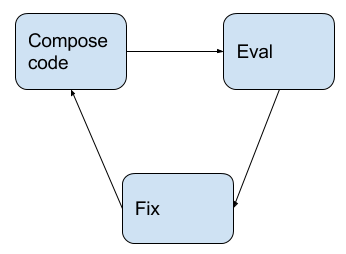
\includegraphics[scale=0.5]{img/Programming.png}
  \caption{Clojure coding cycle}
\label{fig:clojure-coding}
\end{figure}

First, a programmer composes a code from already available functions (either
defined in his project, or other libraries).
Then the code is sent to the interpreter (inside the editor) and the results are
displayed for inspection.
Integrating evaluation into the coding cycle enables the programmer to
immediately see the results and find the errors.
It also enables him to experiment and even find documentation in REPL, instead
of using external tools.
Then, the errors can be fixed or a different modification can be introduced.
This approach poses several challenges.
First of all, already defined functions should be listed for the programmer and
there should be a possibility of easily adding them to the currently composed
code.
Secondly, evaluation and displaying of the results should be built into the
editor.
Furthermore, there should be a way of editing an already evaluated code and
re-evaluating it.
Last but not least, all this code must be presented in a readable manner, as a
diagram of sorts.

\section{Representation}
The most basic functionality of Jarvis is displaying the code as a diagram.
Language primitives are shown as a text, while S-expressions are
represented as boxes \figref{fig:j-box}.
Colors are used to signify different types.
This creates a representation consisting of embedded boxes with textual nodes as
leaves.
For example, a function’s definition
\begin{lstlisting}
(defn inc [num] (+ num 1))
\end{lstlisting}
looks like a box
with two smaller boxes inside.
This has an advantage of presenting S-expressions in a concise way, which is
more readable than parentheses.

\begin{figure}[hbt]
  \centering
  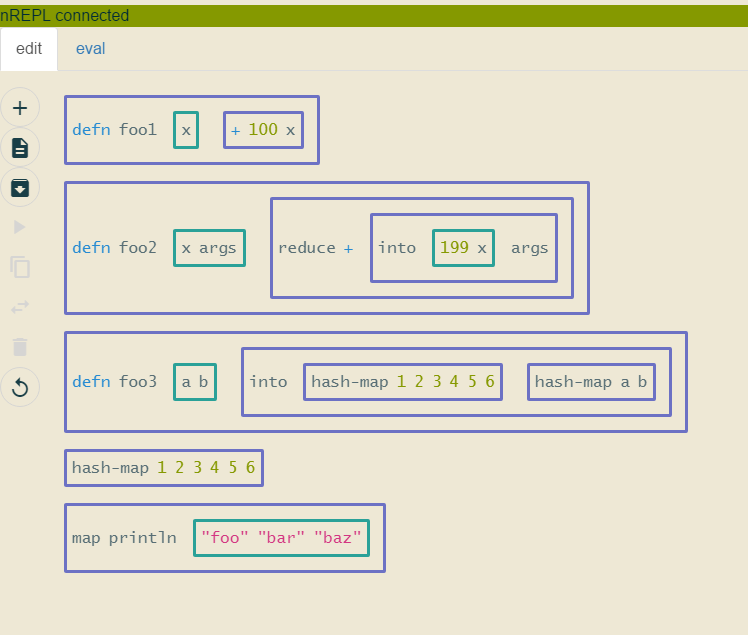
\includegraphics[scale=0.3]{img/j-boxes_f}
  \caption{S-Expressions as boxes in Jarvis}
\label{fig:j-box}
\end{figure}

\section{Modification}
Modification of a code is implemented as two modes --- normal and pasting.
It works in a fashion similar to drag \& drop --- the first click focuses the element.
Then, the user can either pick it up, or copy it and the editor enters the
pasting mode.
Then, the second click inserts the element into given place and the editor
returns to the normal mode.
In the pasting mode possible placement options are shown as buttons
\figref{fig:j-insert}.
All clickable elements are highlighted when cursor hovers upon them.
Additionally, in the pasting mode, options related to the currently picked up
node are available --- this enables the user to delete it or evaluate it.


\begin{figure}[hbt]
  \centering
  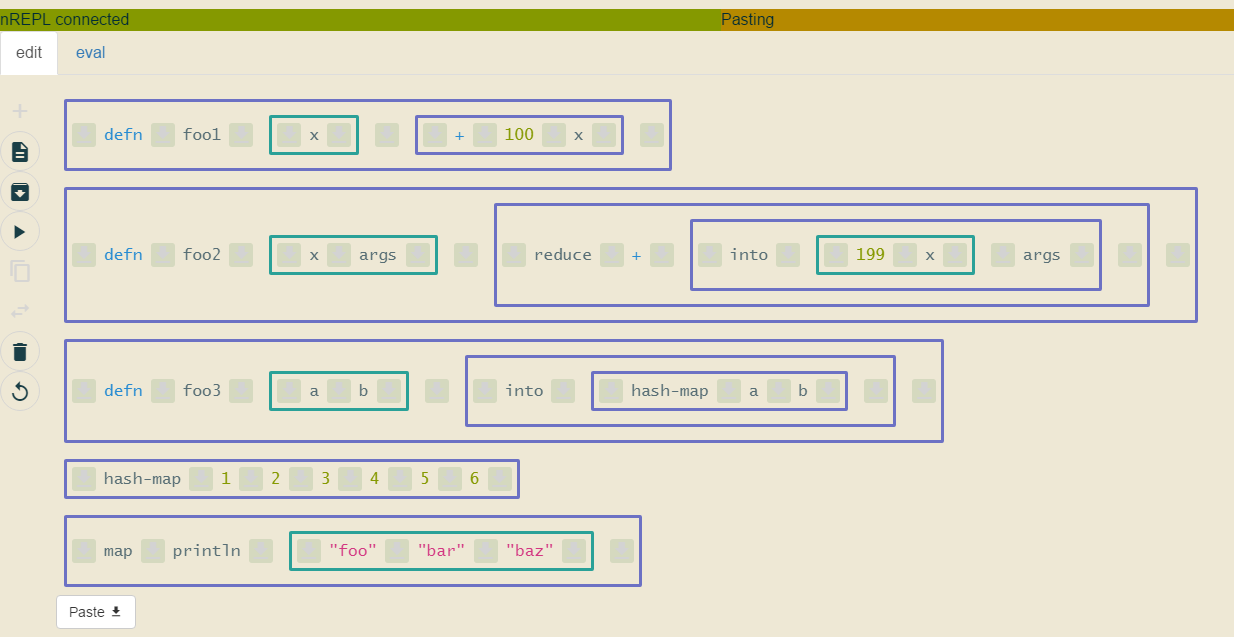
\includegraphics[scale=0.3]{img/j-insert_f}
  \caption{Insert mode in Jarvis}
\label{fig:j-insert}
\end{figure}

\section{Evaluation}
Code evaluation is solved by providing a second tab in which user can see all
previously evaluated expressions.
Upon clicking the evaluation button, the node is moved to the evaluation tab and
the results of evaluating the expression are displayed \figref{fig:j-eval}.
When a user clicks a node in the evaluation tab, it’s moved back to the editing
tab.
This allows the user to rapidly switch between the tabs, running and fixing
code.


\begin{figure}[hbt]
  \centering
  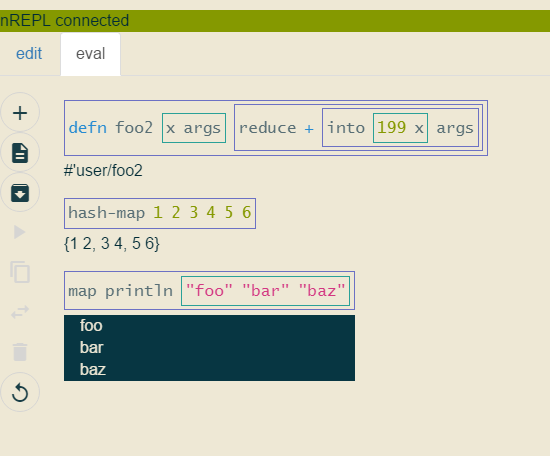
\includegraphics[scale=0.3]{img/j-eval_f}
  \caption{Evaluation tab in Jarvis}
\label{fig:j-eval}
\end{figure}

\section{Installation}
Jarvis is available for several platforms from website
\url{https://scoiatael.github.io/Jarvis}. These include OSX, Windows (both
tested), and several Linux distributions (not tested, with underlying build tool
still not production-ready) \figref{fig:j-inst}.

In order to evaluate the code, Jarvis requires Leiningen
(\url{https://leiningen.org/}).
If it is not found, an error message is shown during the startup
\figref{fig:j-error}. Most of the functionality will continue to work, but any attempts
to evaluate code will result in an error.

\begin{figure}[hbt]
  \centering
  \begin{minipage}{0.48\linewidth}
    \centering
    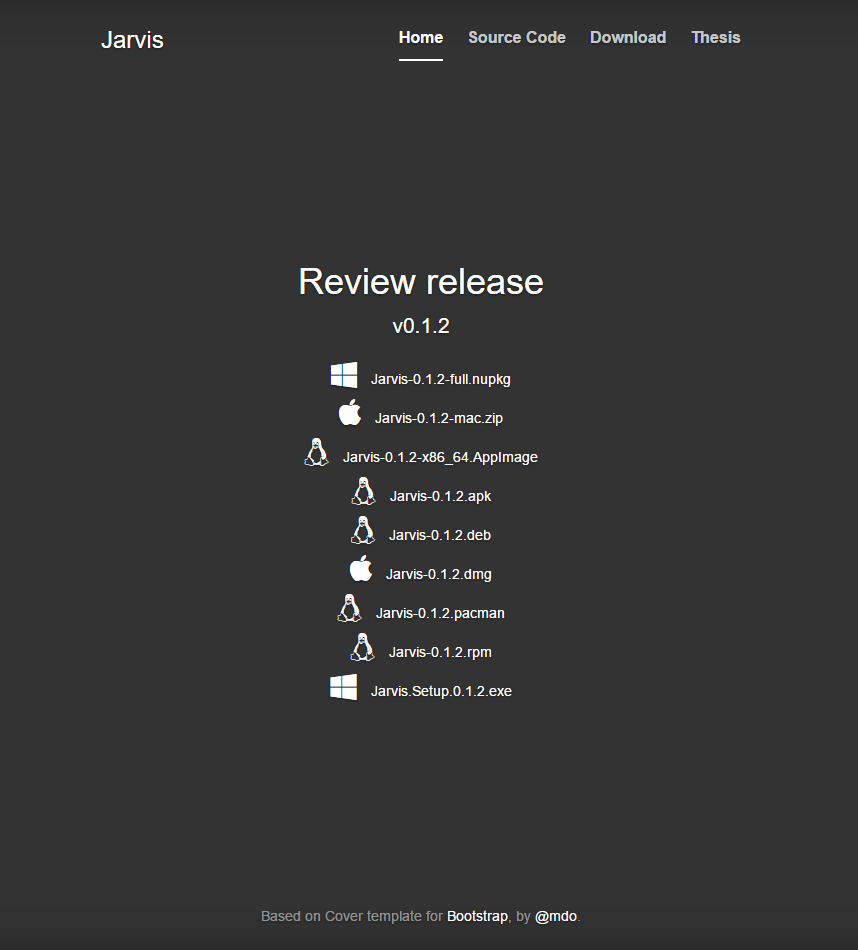
\includegraphics[width=0.9\linewidth]{img/j-inst}
    \captionof{figure}{Download page for Jarvis}
\label{fig:j-inst} 
  \end{minipage}%
  \begin{minipage}{0.48\linewidth}
    \centering
    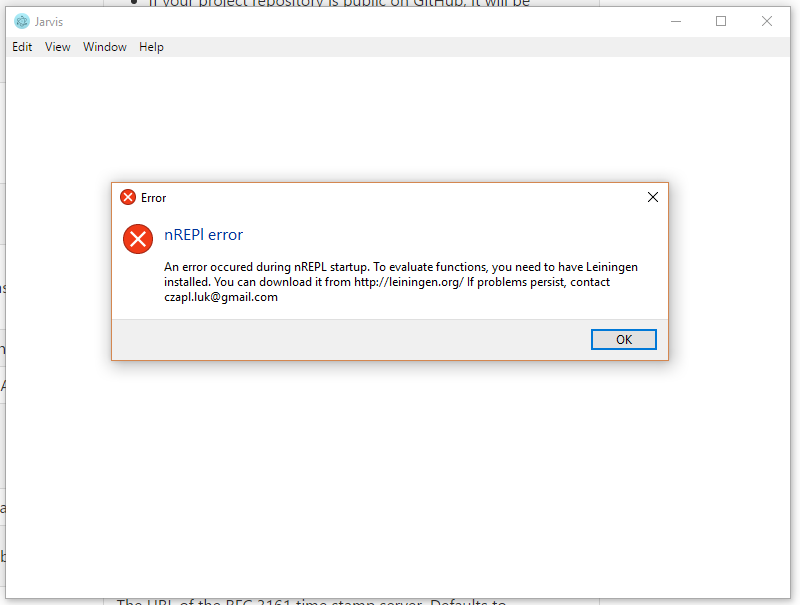
\includegraphics[width=0.9\linewidth]{img/j-error}
    \captionof{figure}{Leiningen not found error}
\label{fig:j-error}
  \end{minipage}
\end{figure}

\section{Example}
In this section we'd like to present writing a simple Fibonacci function in Jarvis.
After starting Jarvis, the user is presented with a blank screen. He can open a file, or
start writing the code \figref{fig:j-startup}. 

\begin{figure}[hbt]
  \centering
  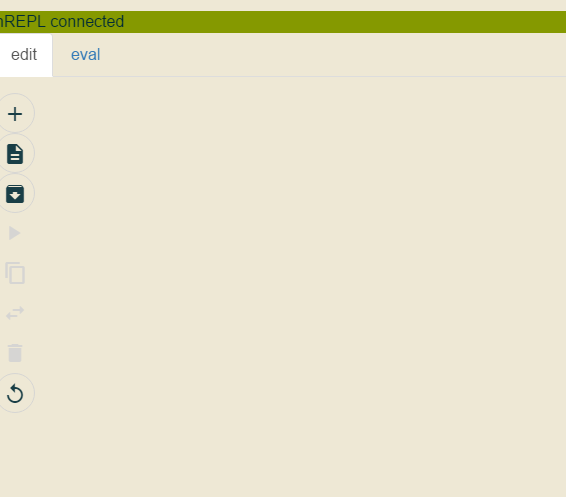
\includegraphics[scale=0.3]{img/j-startup}
  \caption{Empty view after opening Jarvis}
\label{fig:j-startup}
\end{figure}

New elements can be added with \textit{Add element} button \figref{fig:j-add}.
It opens a menu with a searchable list of all functions in
\lstinline{clojure.core}, all
functions defined in the current namespace, some commonly used constructs, and a text
box which user can utilize to add custom elements \figref{fig:j-add_box}.

\begin{figure}
  \centering
  \begin{minipage}{0.48\textwidth}
    \centering
    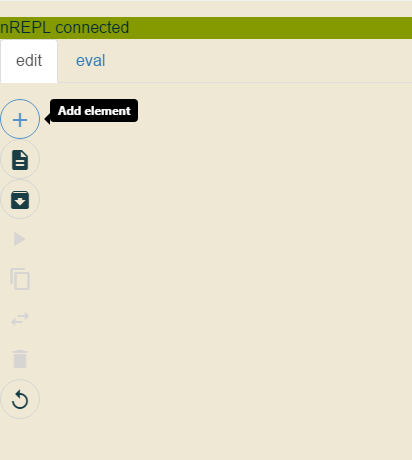
\includegraphics[scale=0.3]{img/j-add}
    \captionof{figure}{Add element button}
\label{fig:j-add}
  \end{minipage}
  \begin{minipage}{0.48\textwidth}
    \centering
    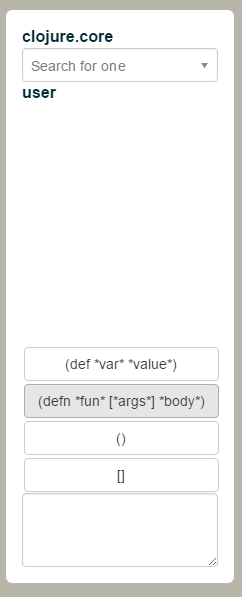
\includegraphics[scale=0.3]{img/j-add_box}
    \captionof{figure}{Add element menu}
\label{fig:j-add_box}
  \end{minipage}
\end{figure}

We'll use it to add \lstinline|defn| --- a function definition. This will create a
node which corresponds to the head of the function definition. It also requires a name of
the function and a vector of arguments. We'll use the text box to add a node containing
\lstinline|fib| --- the function name, \lstinline|[]| --- an empty vector of function
parameters, and \lstinline|i| --- the sole function argument \figref{fig:j-fib_parts}.

Now, we can start gluing these parts together. First, we focus the \lstinline|i| node
with a single click \figref{fig:j-cut}, and then we use the \textit{Cut} button to
remove that node from its current
position and enter the pasting mode \figref{fig:j-pasting}.

\begin{figure}[hbt]
  \centering
  \begin{minipage}{0.48\textwidth}
    \centering
    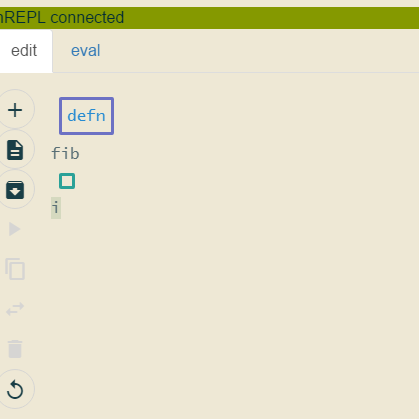
\includegraphics[scale=0.3]{img/j-fib_parts}
    \captionof{figure}{Basic parts of \lstinline{fib} function definition}
\label{fig:j-fib_parts}
  \end{minipage}
  \begin{minipage}{0.48\textwidth}
    \centering
    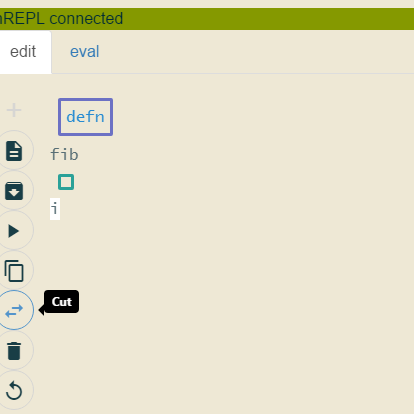
\includegraphics[scale=0.3]{img/j-cut}
    \captionof{figure}{Cut button}
\label{fig:j-cut}
  \end{minipage}
\end{figure}

\begin{figure}[hbt]
  \centering
  \begin{minipage}{0.48\textwidth}
    \centering
    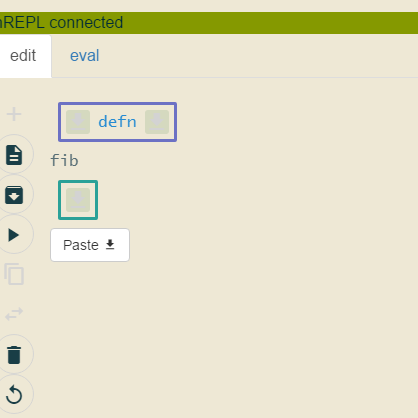
\includegraphics[scale=0.3]{img/j-pasting}
    \captionof{figure}{Pasting mode}
\label{fig:j-pasting}
  \end{minipage}
  \begin{minipage}{0.48\textwidth}
    \centering
    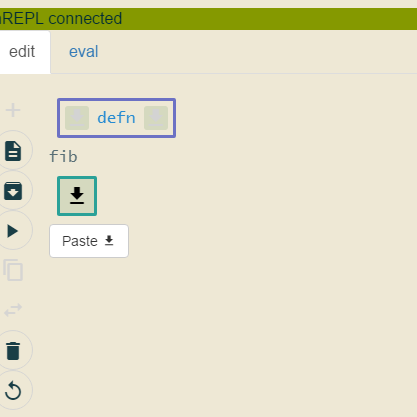
\includegraphics[scale=0.3]{img/j-insert-click}
    \captionof{figure}{Inserting \lstinline{i} into vector}
\label{fig:j-i-insert}
  \end{minipage}
\end{figure}

In the pasting mode, we can click inside the green square (which represents the empty vector) to insert
\lstinline|i| \figref{fig:j-i-insert}.
This ends our work with the vector of parameters \figref{fig:j-inserted}.
Using the same mechanism, we finish the head of the function definition. Then we use
the \textit{Eval}  button to check for potential errors \figref{fig:j-defn-eval}.

\begin{figure}[hbt]
  \centering
  \begin{minipage}{0.48\textwidth}
    \centering
    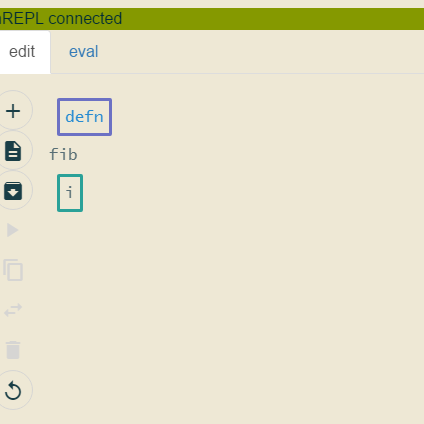
\includegraphics[scale=0.3]{img/j-inserted}
    \captionof{figure}{Finished vector of parameters}
\label{fig:j-inserted}
  \end{minipage}
  \begin{minipage}{0.48\textwidth}
    \centering
    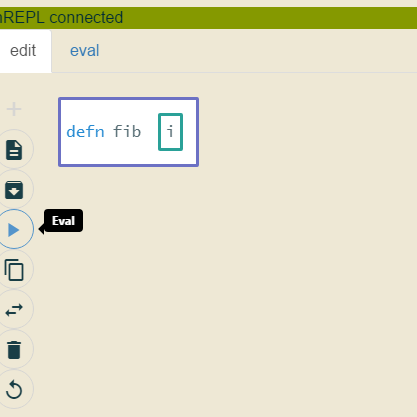
\includegraphics[scale=0.3]{img/j-defn-eval}
    \captionof{figure}{Eval button}
\label{fig:j-defn-eval}
  \end{minipage}
\end{figure}

In the evaluation window we see that no errors were emitted
\figref{fig:j-defn-eval-result} --- so far our function
definition is correct.
Now, we click on the function definition to return it to the \textit{Edit} tab. In
there, we add a simple
\lstinline{if} element \figref{fig:j-if}.
After moving it inside \lstinline{defn} we can check again if errors have been
made \figref{fig:j-if-check}.
Then we proceed to create the second branch of the \lstinline{if} expression ---
a recursive call to \lstinline{fib} \figref{fig:j-fib-rec}.

\begin{figure}[hbt]
  \centering
  \begin{minipage}{0.48\textwidth}
    \centering
    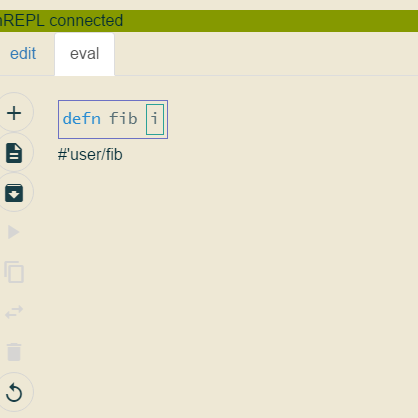
\includegraphics[scale=0.3]{img/j-defn-eval-result}
    \captionof{figure}{Evaluated function definition}
\label{fig:j-defn-eval-result}
  \end{minipage}
  \begin{minipage}{0.48\textwidth}
    \centering
    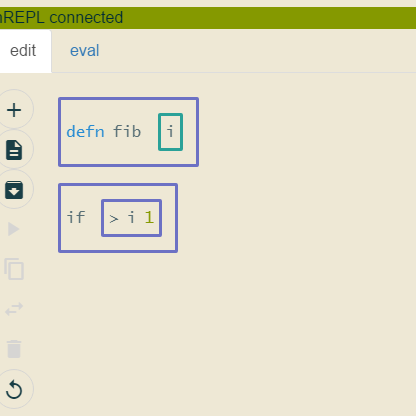
\includegraphics[scale=0.3]{img/j-if}
    \captionof{figure}{Simple \lstinline{if} node}
\label{fig:j-if}
  \end{minipage}
\end{figure}


\begin{figure}[hbt]
  \centering
  \begin{minipage}{0.48\textwidth}
    \centering
    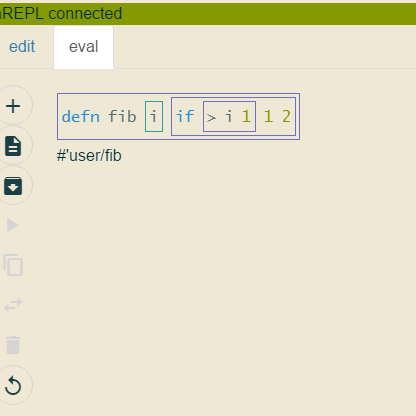
\includegraphics[scale=0.3]{img/j-if-check}
    \captionof{figure}{Evaluated definition with \lstinline{if} body}
\label{fig:j-if-check}
  \end{minipage}
  \begin{minipage}{0.48\textwidth}
    \centering
    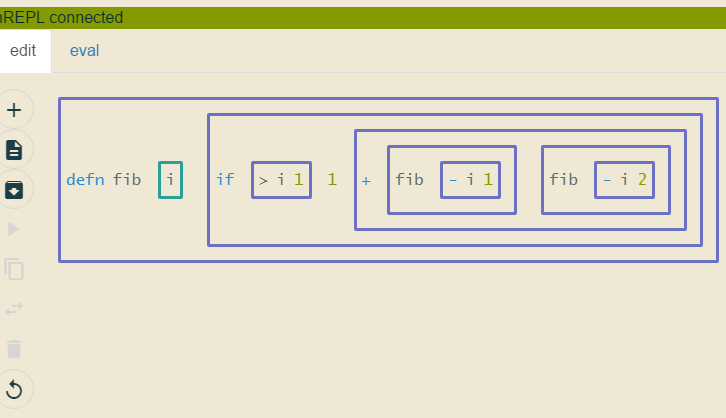
\includegraphics[scale=0.3]{img/j-fib-rec}
    \captionof{figure}{\lstinline{fib} function ready}
\label{fig:j-fib-rec}
  \end{minipage}
\end{figure}

It seems we are finished with our function definition --- now we can
evaluate it again, and check if it
works. We create a simple invocation --- \lstinline{(fib 0)}, and we evaluate it
\figref{fig:j-fib-err}.

It seems there's an error in our definition --- comparison is wrong! We need to
change \lstinline{>} to \lstinline{<}. This can be done easily by adding a new
element via text box, cutting it and pasting in place of the other. Then we can
check if the function indeed works as intended \figref{fig:j-fib-works}.

\begin{figure}[hbt]
  \centering
  \begin{minipage}{0.48\textwidth}
    \centering
    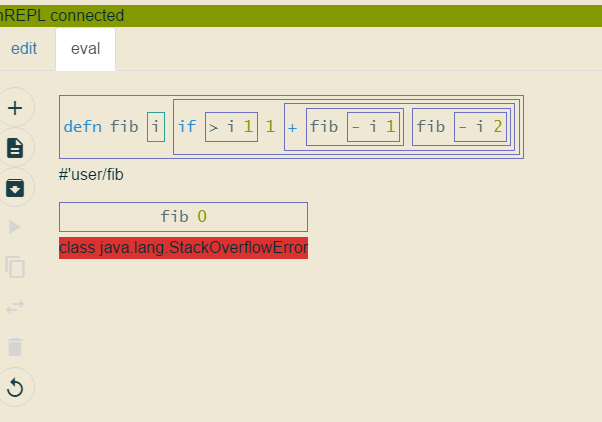
\includegraphics[scale=0.3]{img/j-fib-err}
    \captionof{figure}{Stack overflow error in testing}
\label{fig:j-fib-err}
  \end{minipage}
  \begin{minipage}{0.48\textwidth}
    \centering
    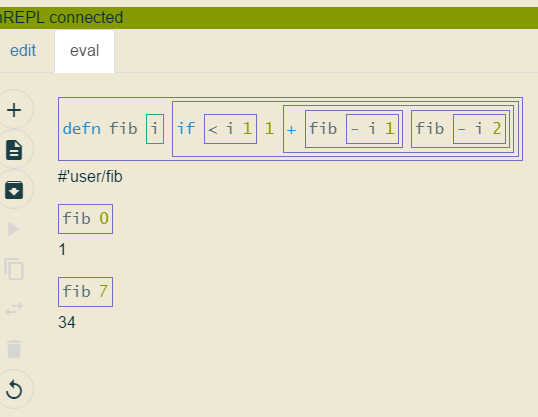
\includegraphics[scale=0.3]{img/j-fib-works}
    \captionof{figure}{Final tests of our Fibonacci function}
\label{fig:j-fib-works}
  \end{minipage}
\end{figure}

\section{Pros and cons of the current solution}
Switching between the normal and ``pasting'' representation is not very intuitive
--- the code appears to ``jump.''
An alternative solution might be to show placement locations at all time --- this
has the disadvantage of requiring a much larger screen in the normal mode.
Another possibility could be to open a new window for pasting.
For example, the user first picks into which top-level expression he wishes to
insert the code, which opens a window with only placement possibilities inside
that expression shown.

Moving the code between evaluation and editing tabs might also be surprising to
some users --- they might think that the code sent to evaluation is somehow lost.
Another solution might be to use more tabs --- one for editing, one for
evaluation, and one for the finished code.
Separate tabs would then represented the three stages of coding: in
progress (editing tab), being tested (evaluation tab), and done (finished tab).
The user should be able to move it both forwards and backwards (to fix or refactor
code).
This has a rather serious disadvantage of cluttering the interface with
unnecessary movement actions (with a possibility of errors and confusing the
user).

Another confusing part about the evaluation are side-effects in REPL --- if a user
evaluates a code, and then moves it to the editing tab, REPL is not cleaned up.
All side-effects accumulate, and thus re-evaluating even the same code might
yield different results.
To solve this, user can force REPL to restart (thus cleaning it up).
An alternative solution might involve a wrapper around REPL, which would gather
all side-effects of evaluation and clean them up if a node is sent back to
the editing tab.


\chapter{Jarvis implementation}
\section{General Architecture}
\subsubsection{Why in Clojure?}
The biggest advantage of using Clojure for this project are users understanding
the codebase.
Writing an editor for Clojure in Clojure ensures that if someone uses it, they
can also contribute to this project.
Potentially, this could mean that even a newcomer might write an extension to
Jarvis in Jarvis itself.
Because of the dynamic nature of the language, this could even lead to people
modifying their editors at run-time! This might make the editor as extensible as
Vim or even Emacs.

Secondary gains include a strong suite of existing libraries (which will be
presented later) and being a functional language.
In this chapter, I’d like to showcase and justify the architectural decisions
behind Jarvis.

\subsubsection{Single source of truth}
State of the whole application is contained in one single Clojure atom, which
can be thought of as a database.
This way every change in the application maps to a change in this atom.
Why is it handy?
\begin{itemize}
\item Debugging. If a list of actions leads to a bug showing up, and changes in
  the state are recorded, the bug can easily be reproduced. Those diffs
  (changes) can be serialized and sent to the programmer for debugging purposes.
\item Understanding the application. Almost every complex application is a state
  machine under the hood, but very few are explicit about it. With the atom
  containing the whole state of application, such is the case with Jarvis. It
  means you can understand the logic behind the whole application by reading the
  list of state transitions.
\item Ease of programming. Having a centralised state
  means that almost every part of the application can be a function of this
  state. Views are functions from state to representation that user sees (HTML
  in this aspect). User action handlers are functions from state and action to
  new state.
\end{itemize}

\subsubsection{One-way dataflow}
Currently, one of the most widespread architectures is Model--View--Controller.
Model is responsible for business logic, View for user interaction, and
Controller is a bridge between them \figref{fig:mvc}.
This has numerous disadvantages as an architecture for a big application,
because it was meant for small components~\cite{Krasner:1988:CUM:50757.50759}!

\begin{figure}[hbt]
  \centering
  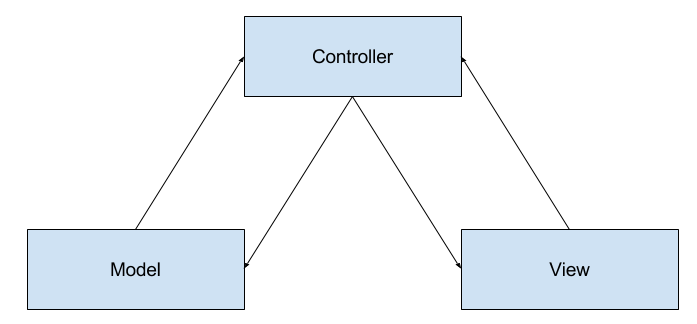
\includegraphics[scale=0.25]{img/MVC}
  \caption{Model--View--Controller}
\label{fig:mvc}
\end{figure}

Recently, it has been criticised and an alternative is being searched for.
One proposal comes from Facebook: it’s Flux architecture.
It can be summed up as an unidirectional data flow.
In traditional MVC one action might affect multiple models, which in turn might
cause more updates in other models.
These cascading updates make the application harder to understand.
Flux takes an approach that bears resemblance to functional reactive
programming.
View renders denormalized data which is obtained from the current application
state.
Ideally, both views and query for data would be declarative.
User (and external inputs, like REPL) triggers actions, which are in turn
reconciled with current application state --- triggering an update of views
\figref{fig:oneway}.

\begin{figure}[hbt]
  \centering
  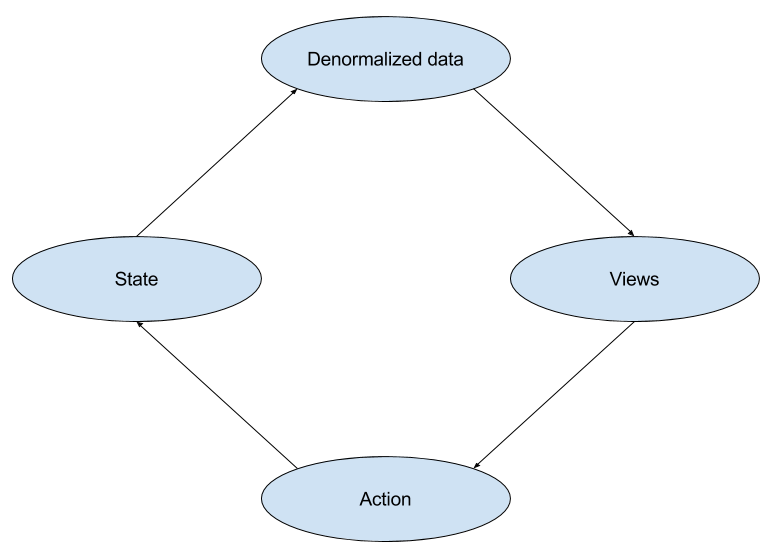
\includegraphics[scale=0.25]{img/OneWay}
  \caption{One way data flow}
\label{fig:oneway}
\end{figure}

\chapter{Implementation internals}
\section{Technologies:}
Jarvis is build on top of technologies that a modern editor, Atom
(\url{https://atom.io/}), uses.
These technologies consist of Chromium rendering engine and Node.js runtime ---
known as Electron (\url{http://electron.atom.io/}).
They allow creating cross-platform desktop applications using Web technologies ---
HTML, JavaScript and CSS.\@
To avoid actually having to write HTML, CSS and Javascript, ClojureScript is
used instead.
It’s Clojure compiled to Javascript.
Coupled with extensions allowing for CSS and HTML generation, it allows to write
a whole desktop application using the best Web libraries in only one language ---
Clojure.

Most of the architectural boilerplate is provided by Re-frame
(\url{https://github.com/Day8/re-frame}).
Efficient, declarative views are provided by Reagent
(\url{https://github.com/reagent-project/reagent}), which uses Facebooks React
(\url{https://facebook.github.io/react/}) under the hood.
CSS is generated using Garden (\url{https://github.com/noprompt/garden}).
Additionally, many smaller libraries are included:
\begin{itemize}
  \item Re-com (\url{https://github.com/Day8/re-com}) --- GUI components for
    Reagent,
    
  \item Figwheel (\url{https://github.com/bhauman/lein-figwheel}) --- hot code
    reloader for development,
    
  \item Schema (\url{https://github.com/plumatic/schema}) --- data description and
    validation library.
    
\end{itemize}

\section{Limitations}
In its current form, Jarvis has several limitations.
Some of them exist due to the nature of the language, and overcoming others
would simply take too much time to implement.
One of the latter cases is the simplicity of the checker --- although Clojure’s
basic syntax is just S-expressions, there is a number of predefined functions
commonly used --- for example \lstinline|defn| used for function definition.
In its most basic form, it accepts a symbol, then a vector of symbols and an
S-expression.

\vspace{5mm}
\texttt{(defn \colorbox{blue!30}{foo} \colorbox{green!20}{[bar1 bar2]} \colorbox{red!10}{(baz (+ bar1 bar2))})}
\begin{itemize}
  \item \texttt{\colorbox{blue!30}{foo}} --- function namespace
  \item \texttt{\colorbox{green!20}{[bar1 bar2]}} --- vector of formal arguments
  \item \texttt{\colorbox{red!10}{(baz (+ bar1 bar2))}} --- function body
\end{itemize}
\vspace{5mm}

If a part is omitted, runtime error is guaranteed.
To improve user experience, the editor could detect errors in such forms.
Such checker could also find undefined variables and warn about their usage.
It could also check arity of functions.
Currently, such functionality in Jarvis is implemented in a proof-of-concept
manner --- it can detect only the most basic forms of \lstinline|defn|,
\lstinline|fn|, \lstinline|def|, \lstinline|let|. These cover most of Clojure
“types” of introducing scope and defining variables and functions.

Another big limitation is the lack of support for data structures other than
list and vector.
This doesn’t limit functionality (as any Clojure program can be written by using
their constructors, instead of literals --- e.g. \lstinline|(hash-map 1 2)|
instead of \lstinline|{1 2}|),
but doesn’t provide a good user experience.
The same goes for reader forms --- for example, lambda-abstraction syntax
(\lstinline|#(+ 1 2)|
instead of \lstinline|(fn [] (+ 1 2))|) is not parsed correctly.

The third limitation is the lack of support for macro operators.
Although instead of using \lstinline|'| (quote) user can user quote function, there is no
such equivalent for \lstinline|`| (syntax quote), \lstinline|~| (unquote) and
\lstinline|~@| (unquote splice).
Additionally, Jarvis has no knowledge of macros --- they can be used and defined,
but that’s hard due to the quoting limitations.
Jarvis has also no knowledge of Clojure module system --- it currently only lists
functions in the current namespace, and those in \lstinline|clojure.core|.
Users would greatly benefit from Jarvis being able to list all of the namespaces
available, adding them to the current project, and being able to search and
insert variables from any namespace found.


\section{Possibilities of future extensions}
There are several possibilities of extending Jarvis in the future, besides
removing the limitations listed in the previous section.
The first of them is embedding a Clojure interpreter inside Jarvis, so that it
can be directly extended in Clojure --- much like Emacs and ELisp work right now.
This would allow to add new features and modify existing ones at runtime,
allowing users to create extensions (instead of having to add new features
directly).
Over the years, this has proved a sound strategy for open source editors.
Another experiment could be different code representations --- current box
representation isn’t innovative --- tree or graph representation might turn out to
be more readable.
Even switching between them at run-time could be implemented.

Yet another possibility is creating a mobile (targeted for tablets) version of
Jarvis.
This would require using embedded Clojure instead of running REPL (as it is
right now), but would enable a whole new range of devices for which Jarvis would
be uniquely suited because of touchscreens.
Improving code manipulation is also an option --- the current drag \& drop
interface is not very user-friendly.
If combined with more complex checkers, one might detect in which points code
can (or should) be added and provide easy visual cues for users.


\chapter{Jarvis and other VPLs}
\section{Other major VPLs}
\subsubsection*{Scratch}
Scratch is a VPL designed for educational purposes by the Lifelong Kindergarten
Group at the Massachusetts Institute of Technology (MIT).
It uses a block-based approach \figref{fig:scratch}.
Individual elements of the language are represented as pieces of jigsaw puzzles
and fit together in different combinations.
Drag \& drop is a primary method of assembling them, with details tweaked by
secondary input options (like paint or sound editor) and text (for numbers and
strings).

\begin{figure}[hbt]
  \centering
  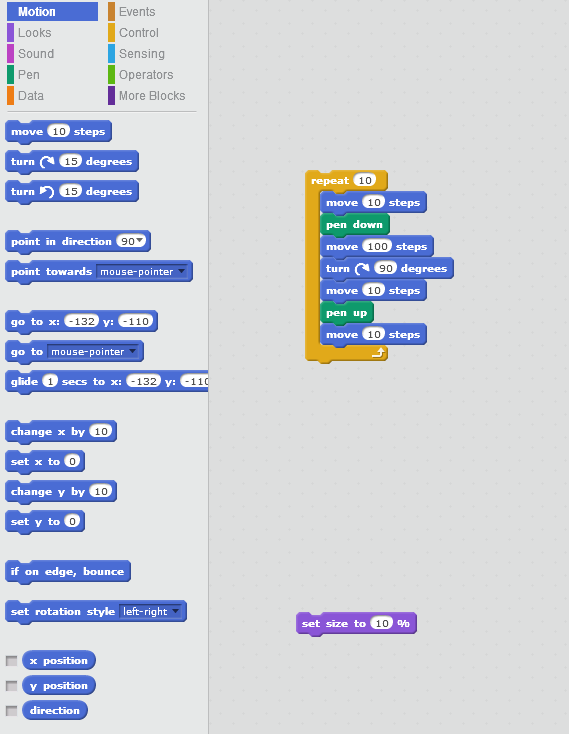
\includegraphics[scale=0.3]{img/s-puzzle}
  \caption{Scratch editing window}
\label{fig:scratch}
\end{figure}

\subsubsection*{Blueprints}
Blueprints Visual Scripting is part of Unreal Engine 4, developed by Epic Games.
It aims to help designers and developers help in processes that have
traditionally been done by programmers.
Interface is node-based --- each one represents a part of the language (like a
function call), with wires connecting them \figref{fig:blueprints}.
Wire can represent either control or data flow, with both being present in a
single script.
For example \lstinline|if| has one control wire and one data wire coming in (execution
flow and boolean value), and two control wires coming out (one for \lstinline|then|, and
one for \lstinline|else| flow).
Developers are expected to manipulate nodes and wires with mouse, while
underlying implementation for nodes should be provided by programmers as text.

\begin{figure}[hbt]
  \centering
  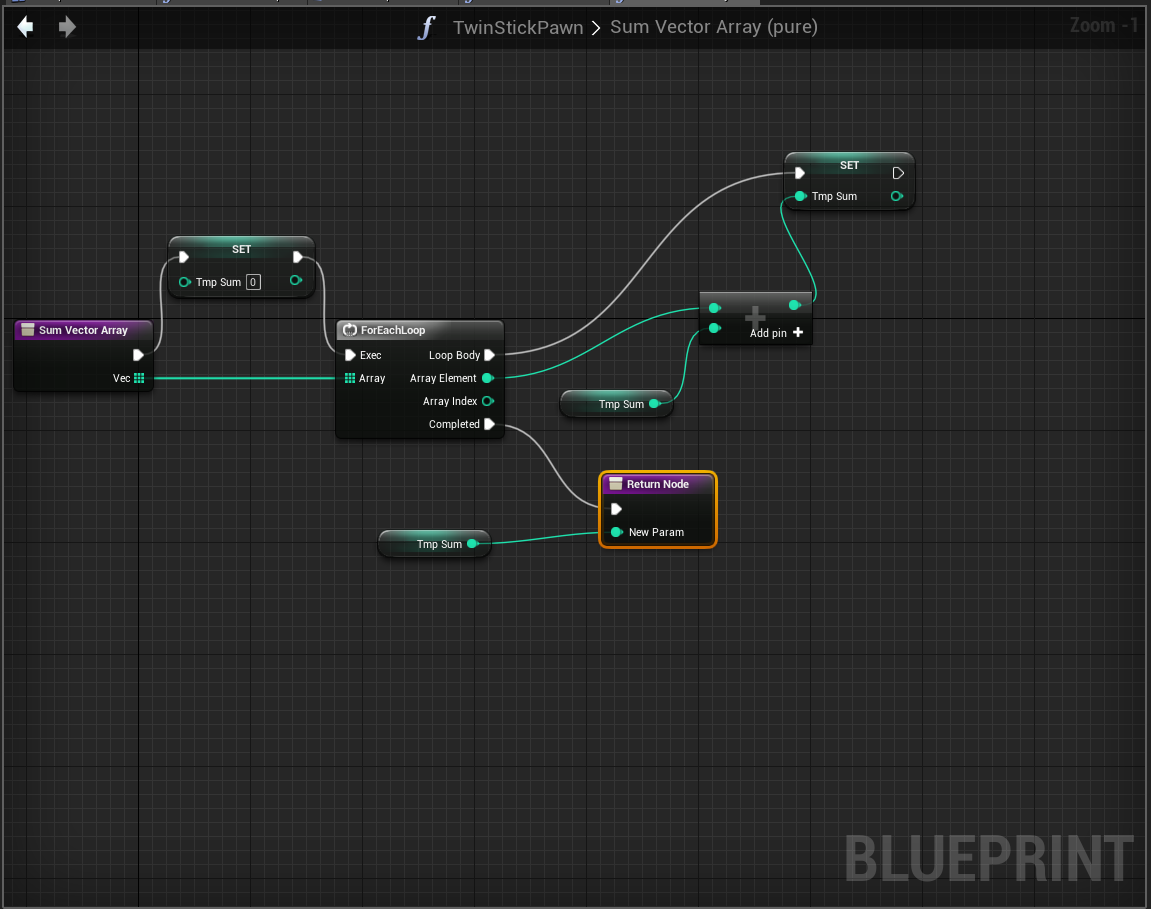
\includegraphics[scale=0.3]{img/b-wires}
  \caption{Blueprints}
\label{fig:blueprints}
\end{figure}

\section{Features}

\subsubsection*{REPL integration}
Many traditional editors (like Emacs, VIm, or Lighttable) offer possibility to
execute parts of the program directly from editor, increasing programmers ability to
debug program before its fully written.
Both Jarvis and Scratch have the same capability, but Blueprints does not
possess it. That is caused by Unreal editor model of creating full scenes before
running it. Possibly professional programmer would only need to debug
scene-by-scene, instead of parts of programmer, but for a novice this proves
difficult.

\subsubsection*{Representation}
Jarvis represents the program as a series of boxes, each representing data structure
in Clojure. Scratch uses similar representation --- expressions are boxes, and
those which can interact (as for example conditional expression, and boolean
condition) can interlock, allowing the programmer to intuitively understand the
underlying type system. Blueprints uses nodes (represented by boxes) connected
by wires, which represent data and control flows. This offers the programmer
even better understanding of the language, but is quite difficult to
manipulate and get used to.

\subsubsection*{Holes}
Both Scratch and Blueprints offer suggestions where some pieces may be missing
(by showing respectively empty holes and dangling endings). Of these two Scratch
is better. Jarvis does not offer any such insight --- that is due to Clojure
functions having possibly multiple arities. Such errors are left to be caught
during evaluation in REPL.\@

\subsubsection*{Comments}
Comments increase the chance of readers understanding the program. Blueprints allow placing
comments on groups of nodes. Scratch and Jarvis have no such capability.

\subsubsection*{Manual placement}
In both Blueprints and Scratch, programmer is expected to place parts of
a program manually. That creates a potential source of problems --- the programmer has
to worry how his changes would affect the placement of the whole program. In Blueprints,
this problem is partially alleviated by automatic re-wiring --- if two nodes
were connected, the programmer can freely move each of them, and they will still be
wired together. Jarvis has fully automatic placement, dictated by the structure of
the underlying Clojure program. 

\subsubsection*{Functions}
The ability to group and parameterize code gives the programmer a very important tool to
avoid code duplication. All three editors offer such
possibility, which is least emphasized in Scratch (due to its simplicity) and
most in Jarvis (due to Clojure being a functional language).

\subsubsection*{Modules}
Building on what functions offer, modules help organize groups of functions.
Scratch doesn't possess modules, but Jarvis and Blueprints do. The support for them
in Jarvis is limited (the programmer can import and use functions from the other
modules, but they are not listed like functions from current namespace --- which
is the Clojure term for ``module'').
Blueprints has no such problems --- the programmer can easily see and use functions
from the other modules.

\section{Using HCI approach}
While a list of features helps understand what the exact low-level
differences between the editors are, in order to better understand what makes one
better or worse, a different kind of approach is needed.
In his work Green presents a framework called “cognitive dimensions
of notations” for assessment of cognitive artefacts.
It can be used to compare VPLs~\cite{Green96UsabilityAnalysis}. In this section,
we’ll use this framework to compare Jarvis with Scratch and Blueprints.

\subsubsection*{Abstraction Gradient}
Abstraction is:
\blockquote{Grouping of elements to be
  treated as one entity, whether just for convenience or to change the
  conceptual structure~\cite{Green96UsabilityAnalysis}.}
This criterium segregates interfaces based on the flexibility of the
representation and the requirements on the programmer for adapting.
For example, simple control flow diagrams that are often used in place of a
pseudo-language to define an algorithm, and state machines, can be categorised
as abstraction-hating.
Using them, meaning can be defined quickly, but adding new elements is
challenging and requires a lot of explaining.
On the other end of the spectrum are interfaces which require programmers to
define their own abstractions (and thus make each program a unique challenge to
a newcomer).
Functional languages are the prime example.
Each new function acts as an abstraction.
The program itself is built as an abstraction over more abstractions (akin to a
pyramid).
This category is named abstraction-hungry.
Middle-ground between them is labeled as abstraction-tolerant (Pascal or Python
are the prime examples).

Scratch is abstraction-tolerant --- new abstractions can be defined in form of
custom blocks, but a novice programmer can easily go on without doing so.
On the other hand, both Blueprints and Jarvis are abstraction-hungry.
That’s caused by both node (in Blueprints) and box (in Jarvis) being an
abstraction over some function.
Both approaches are very similar from the following point of view.
A novice programmer has some traditional primitives (conditionals, loops,
arithmetic) available, but is expected to build a couple of his own abstractions
on top of others.

\subsubsection*{Closeness of Mapping}
Solving a problem can be easy in terms of a problem world, but very hard in
terms of a program world.
For example, turning car right is easy when you are a driver, however writing a
program that turns car right depends on the abstraction given to you by both
your language and interface of a car programming.
Domain specific languages are designed to solve this problem --- to allow
programming in terms of the problem world.
VPLs are also pretty good at this, because they are often developed to map to
one domain.
Scratch has a clearly defined problem world (moving objects on screen) and its
mapping is very close, with (almost) every piece of puzzle representing some
action in the problem world.
For general-purpose languages, that evaluation is much harder.
It requires thinking about a very simple problem world and considering how many
language primitives are needed to solve a problem there.

Here, Jarvis seems to have the upper-hand.
Blueprints require additional wiring of control flow, and many nodes associated
with manipulation of local variables.

\subsubsection*{Consistency}
A notion of language being consistent or not is hard to define objectively.
Inconsistencies for end-users might arise as a result of a very consistent
approach from the language designer.
One might argue that the simplest way to avoid such inconsistencies is making
the language as simple as possible.
The comparison of Scratch, Blueprints and Jarvis does support that claim: all
three have a much simpler structure than textual languages and no
inconsistencies are present.
Jarvis (because of underlying Clojure) seems to be the best --- with only a
handful of primitives, consistency of everything else is up to the programmer.
Scratch has more language elements, which are grouped by type (represented by
shape) and category (represented by colour).
Blueprints is built on top of primitives provided by the programmer, with only a
representation being defined.

\subsubsection*{Diffuseness/Terseness}
This criterium is hard to measure independently of Closeness-of-Mapping, as
language closer to the problem world will require less primitives to solve it.
Another problem is that the ideal language cannot be either too diffuse or too
terse.
If too terse, the programmer will have a hard time finding bugs, as they may be
virtually invisible.
If too diffuse, programmer has to read and memorise a lot to understand what’s
happening.
For VPLs this is especially important, as the total amount of screen space
needed to represent a program should be taken into account.
Scratch is by far the most terse of the three compared.
Jarvis and Blueprints require much more screen space --- with Blueprints using
different tabs for each function and supporting multiple levels of zoom to allow
the programmer to either inspect the details or focus on a bigger picture.
Jarvis supports two views --- one for program parts being currently edited (which
takes more space, to assist in editing) and one for parts that have already been
executed (which takes less space, to make reading easier).

\subsubsection*{Error-proneness}
Generally, VPLs are much less prone to syntax errors than traditional textual
languages.
Their representation makes it virtually impossible to make a syntax error.
Jarvis uses boxes to save the programmer from trouble with parentheses, the
Scratch jigsaw puzzle makes it impossible to make an error, and Blueprints will
not allow the programmer to wire the program in a wrong way.

\subsubsection*{Hard Mental Operations}
Conditionals and boolean arithmetic are a prime example of a notation gone
wrong.
It’s easy to express an easy-to-grasp idea in an incomprehensible way.
Surprisingly,~\cite{Green96UsabilityAnalysis} shows that although diagrams look
like a good way to avoid such problems, they often fail to do so.
Even if shown as a diagram, conditionals imbued in more conditionals resemble a
visual exercise on a formal logic course, not something easy to grasp.
Scratch suffers the most from this, as it uses imperative programming as its
base.
Blueprints (with Object Oriented programming) is a bit better, and Jarvis (with
functional programming) fares best.
That is solely caused by how often that kind of hard mental operations happen in
underlying programming thinking patterns and not by the representation.

\subsubsection*{Hidden Dependencies}
Hidden dependencies are
\blockquote{Relationships between two
  components such that one of them is dependent on the other, but that the
  dependency is not fully visible~\cite{Green96UsabilityAnalysis}.}

They are caused by side-effects (such as assigning a value to a shared
variable).
Generally, VPLs fare better than textual languages when it comes to low-level
(local) dependencies --- simply because they have more means to visualise that
dependency.
When it comes to high-level dependencies, they don’t seem to fare any better.
So is the case with Scratch and Blueprints, with Jarvis showing more promise.
Both Scratch and Blueprints have global variables, and no good support for
showing where they are modified.
Jarvis (thanks to Clojure), has a better model for handling side-effects, but no
means of visualising it.

\subsubsection*{Premature Commitment}
When solving problems, the programmer should worry about the problem world.
Many programming languages pose many requirements on the structure of the
program, making working with them tiring, as programmer has to cope with a lot
of additional guessing ahead.
This criterion measures how much additional guesswork is associated with solving
problems in the given language.
Generally, VPLs using 2D spatial representations tend to pose less difficulties
than textual languages, but are not without problems themselves.
For box-and-wire languages, the placement of boxes with a minimum number of
wires crossing requires a guess-ahead.
Such is the case with Blueprints.
For Scratch, the problem is with placing puzzles to group them and leaving
enough space for subproblems.
% http://www.grammarbook.com/punctuation/apostro.asp
The Jarvis' problem is similar to the problems of textual languages --- the order
of evaluation.
Parts sent to REPL first are shown first and there’s no way of re-ordering them
(besides moving them back to editing and evaluating later, which places them at
the end).
This makes leaving holes for subproblems impossible, thus the whole program
resembles a tree flattened in a prefix fashion.
Imposing some structuring on such list is challenging, to say the least.

\subsubsection*{Progressive Evaluation}
Some languages forbid running programs that are not complete.
Other --- mostly dynamic interpreted languages allow running parts of a program.
Ideally, the programmer can write a program by interacting with REPL and saving
the working parts.
Such is the case with Jarvis.
The program is constructed by running small expressions and composing them to
solve bigger problems.
Scratch also allows running expressions, but results are shown by changing the
state of stage --- to see them again, you need to re-run the expression.
Blueprints doesn’t allow running any expressions because everything is wired to
a global stage.
You can only run the whole game and observe what changes were introduced by your
code modification.

\subsubsection*{Role-expressiveness}
Generally, programmers agree that \emph{some} languages are harder to read than others.
Unfortunately, there’s no consensus on exactly which of them are.
A C programmer might argue that LISP is an unreadable mess of parentheses, while
his adversary would say that the bloated syntax of C makes understanding even
simplest programs challenging.
To avoid this argument, one can consider how easy it is to understand what a
given expression is for.

\blockquote{Role-expressiveness is presumably
  enhanced by the use of meaningful identifiers, by well-structured modularity,
  by the use of secondary notation to signal functionally-related groupings, and
  by the presence of ‘beacons’ that signify certain highly diagnostic code
  structures~\cite{Green96UsabilityAnalysis}.}

Scratch offers no means of modularity besides defining functions and no
secondary notation besides the placement of blocks.
There are also no diagnostic code structures.
Blueprints allows to add comments to a group of nodes.
Jarvis, on the other hand, has no support for comments, but allows using
Clojure pre- and postconditions to annotate functions with extra information
about arguments and returned values.
This can be additionally extended by using proper Clojure libraries (which can
add such features as types of functions).

\subsubsection*{Secondary Notation and Escape from Formalism}
As discussed before, main secondary notation for VPLs is the spatial placement
of items.
That is only possible in Scratch, with Blueprints supporting additionally
comments.
In Jarvis, the programmer has no secondary means of conveying information.
Indenting and manual placement of items are impossible, comments are not
supported.
The programmer is entirely dependent on language features.

\subsubsection*{Viscosity: resistance to local change}
Programmers tend to make mistakes.
Some are easier to fix than others, which often depends on the language.
The biggest issue of Scratch is the order in which items have to be moved
(generally, moving one item moves the rest below it).
This sometimes imposes a big amount of changes needed to move just one block.
Blueprints has a problem with wiring --- although wires are placed automatically,
changing a block can require moving a lot of other blocks to make the program
readable again.
Jarvis has a problem with shuffling blocks.

\subsubsection*{Visibility and Juxtaposability}
This criterion measures how easy it is to just see what the program does,
without much mental work.
This is tightly coupled with the ability to see different parts of the program
at the same time.

Neither Scratch, Blueprints, nor Jarvis offer such a thing.
Overall, all three VPLs make programmer’s life hard in this aspect, which is
especially shameful for Jarvis, because most Clojure editors allow instantly
looking up the definition of any symbol.
Code navigator would also be a big improvement here.

\chapter{Jarvis and mainstream Clojure editors}
In this section we'll compare Jarvis with other editors commonly used to write
Clojure programs: VIm, Emacs, and Lighttable.

\section{Major Clojure editors}
\subsubsection*{VIm}
VIm (\url{http://www.vim.org/}) is a small but easily extensible editor, first
released in 1991. Clojure editing is improved by several plugins --- some of
them provide REPL support, other offer better means of editing S-expressions.

\subsubsection*{Emacs}
Emacs (\url{https://www.gnu.org/software/emacs/}) is surprisingly not a text
editor --- it is LISP interpreter, with text editing being only one of its
functions. As with VIm, Clojure editing is provided by many plugins, which often
build on top of one another.

\subsubsection*{Lighttable}
Lighttable (\url{http://lighttable.com/}) is a ``next generation code editor.''
It tightly integrates with the edited language, providing means to easily run and
watch program being executed from the editor. One plugin provides integration of
Clojure into Lighttable.

\section{Features}
\subsubsection*{REPL integrations}
All of the compared editors offer the possibility to execute parts of program
directly from the editor.

\subsubsection*{S-expressions editing}
All of compared editors offer the possibility to manipulate S-expressions (using,
amongst other, the techniques described in [Section~\ref{sec:editing}]).
    
\subsubsection*{Project awareness}
Emacs, Lighttable and VIm support multi-file projects, by providing means to
easily switch between files and cross-reference functions. Jarvis focuses
on editing one file, and doesn't offer means of switching edited files easily
(besides opening new file, which closes the current one).
    
\subsubsection*{Refactoring}
All three textual editors offer support for refactoring (renaming, extracting function
definitions, inlining functions). Jarvis has no such capability, although
a programmer should be able to add it quite easily (via REPL integration,
similar to how it is implemented in VIm and Emacs).
    
\subsubsection*{Syntax check}
All textual editors offer ability to detect and present possible errors, in
varying degrees --- with the most basic being the detection of misplaced parentheses.
In this aspect Jarvis proves superior --- the programmer simply cannot make such
a mistake. Jarvis also tries to analyze the code and show possible semantic errors
with the help of REPL.\@
    
\subsubsection*{Autocomplete}
Most textual editors currently in use have the ability to autocomplete identifiers
(to avoid typing full names), either by scanning all words in the current document
or by more sophisticated means. Jarvis connects to REPL and offers the
programmer a list of functions currently available to him.
    
\subsubsection*{Syntax highlighting}
Color-coding different language parts (identifiers, brackets) helps programmer
to understand program structure. VIm, Emacs and Lighttable offer this, but
Jarvis offers more --- it visualizes program as a diagram, which adds another
dimension to the representation. This might prove especially important to novices.
    
\subsubsection*{Automatic indentation}
VPLs often place nodes automatically --- textual editors try to do the same by
automatically indenting the code. It removes the need for programmer to
structure the code by himself. It is present in Emacs, VIm and Lighttable, with
Jarvis offering similar capability by placing all boxes automatically.

\chapter{Summary}
Representing a program written in Clojure --- a language based on LISP's idea of
S-expressions and
data--as--code --- as a diagram proves to be a successful experiment.
Jarvis is a new kind of Visual Programming Environment, one that allows
having all pros of ``programming with diagrams,'' while avoiding downsides
traditionally associated with Visual Programming Languages. This approach, if
developed further, could lead to programming environments using entirely different means
for communication with programmer than keyboard and mouse --- for example
touchscreens.

Compared to traditional Clojure programming environments (Emacs, VIm,
Lighttable), Jarvis lacks features associated with
multi-file projects, but proves superior in representation and error avoidance.
Compared to other VPLs (Scratch, Blueprints), it lacks features that improve
user experience, but generally is on the same level of usability.

In addition, there are many potential development ideas for Jarvis, which could lead
to it becoming a professional programming environment.

\bibliographystyle{alpha}
\bibliography{books}
\end{document}
